\documentclass[12pt]{article}

\usepackage[a4paper,top=3cm,bottom=2cm,left=2cm,right=2cm,marginparwidth=1.2cm]{geometry}
\usepackage{fancyhdr}
\usepackage{float}
\usepackage{tikz}

\author{Your Name}
\title{Analytic Studies and Sampling Techniques}
\date{}

\begin{document}
\pagestyle{fancy}
\lhead{STAT110/115 Tutoring Materials}
\rhead{Contingency Table}

\begin{itemize}
\item \textbf{Relative Risk (RR)}: Ratio of two probabilities. RR gives the risk of an outcome relative to "exposure". It is calculated as the ratio of the risk of an outcome for an exposed and an unexposed group. $$RR = \frac{a/(a+b)}{c/(c+d)}$$
Meaning of the RR value: RR = 1 there is no association between outcome and exposure (e.g. rugby position and injury). RR < 1 first row happens less likely than the second row. RR > 1 first row happens more likely than the second row.
\item \textbf{Risk Difference (RD)}: Difference between two probabilities. The RD is given by the difference in the risk for the two groups. $$RD = \frac{a}{a + b} - \frac{c}{c + d}$$
\item \textbf{Odds Ratio (OR)}: Ratio of two odds. The OR compares the odds of an outcome for two groups. Ratio of the odds of the outcome for the exposed group to that for the unexposed group. $$OR = \frac{a/b}{c/d} = \frac{ad}{bc}$$. There is no mathematical distinction between exposure and outcome variables -> makes it particularly useful for quantifying associations between binary variables where there is no "direction" e.g. alcohol consumption (Yes/No) and smoking (Yes/No).
\item \textbf{Confidence Interval for Difference Between Two Proportions}: $$p1 = \frac{a}{r1}$$, $$p2 = \frac{c}{r2}$$, $$(p_1 - p_2) \pm Z_{(1 - \frac{\alpha}{2})} \sqrt{\frac{p_1(1-p_1)}{n_1} + \frac{p_2(1-p_2)}{n_2}}$$

\item \textbf{Steps to Calculate the Confidence Interval for Relative Risk}:
    \begin{itemize}
    \item Get the RR value.
    \item Get the ln(RR).
    \item Calculate the SE of ln(RR) (with formula).
    \item Calculate the CI for ln(RR) (with formula).
    \item Calculate the CI for RR (exp() function).
    \end{itemize}
\item \textbf{Standard error for Confidence interval for relative risk:}$$S_{ln}(RR) = \sqrt{\frac{1}{a} - \frac{1}{r_1} + \frac{1}{c} - \frac{1}{r_2}}$$
\item \textbf{Key formula for Confidence interval for relative risk:}$$\ln(RR) \pm Z_{(1-\frac{\alpha}{2})} \cdot S_{\ln(RR)}$$
\item \textbf{Steps to Calculate the Confidence Interval for Odds Ratio}:
    \begin{itemize}
    \item Get the OR value.
    \item Get the ln(OR).
    \item Calculate the SE of ln(OR) (with formula).
    \item Calculate the CI for ln(OR) (with formula).
    \item Calculate the CI for OR (exp() function).
    \end{itemize}
\item \textbf{Standard error for Confidence interval for Odds Ratio:} $$S_{\ln(OR)} = \sqrt{\frac{1}{a} + \frac{1}{b} + \frac{1}{c} + \frac{1}{d}}$$
\item \textbf{The meaning for range of CI:}
\begin{figure} [H]
\centering
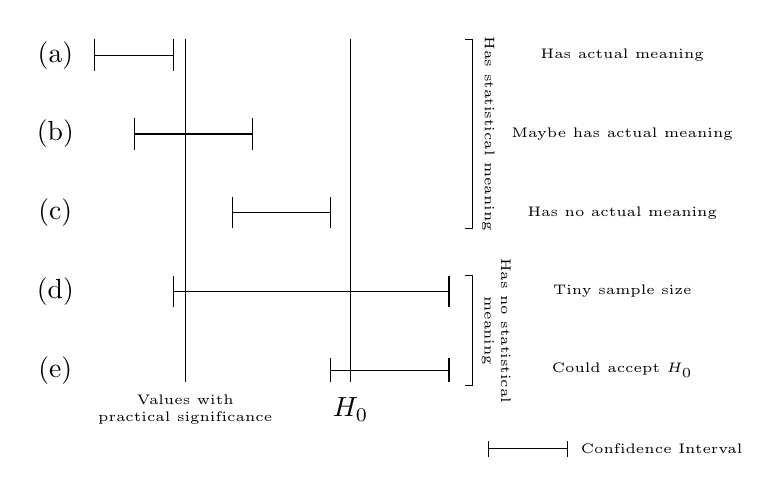
\begin{tikzpicture}
% Horizontal lines with error bars
\draw (0,5) -- (1,5); % Line a
\draw (0, 4.8) -- (0, 5.2); % Error bar for line a
\draw (1, 4.8) -- (1, 5.2); % Error bar for line a

\draw (0.5,4) -- (2,4); % Line b
\draw (0.5, 3.8) -- (0.5, 4.2); % Error bar for line b
\draw (2, 3.8) -- (2, 4.2); % Error bar for line b

\draw (1.75,3) -- (3,3); % Line c
\draw (1.75, 2.8) -- (1.75, 3.2); % Error bar for line c
\draw (3, 2.8) -- (3, 3.2); % Error bar for line c

\draw (1,2) -- (4.5,2); % Line d
\draw (1, 1.8) -- (1, 2.2); % Error bar for line d
\draw (4.5, 1.8) -- (4.5, 2.2); % Error bar for line d

\draw (3,1) -- (4.5,1); % Line e
\draw (3, 0.85) -- (3, 1.15); % Error bar for line e
\draw (4.5, 0.85) -- (4.5, 1.15); % Error bar for line e

\draw (1.15, 0.85) -- (1.15, 5.2); % first bar
\draw (3.25, 0.85) -- (3.25, 5.2); % second bar

% Labels for horizontal lines
\node at (-0.5,5) {(a)};
\node at (-0.5,4) {(b)};
\node at (-0.5,3) {(c)};
\node at (-0.5,2) {(d)};
\node at (-0.5,1) {(e)};

\node [font=\tiny, align=left] at (6.7, 5) {Has actual meaning};
\node [font=\tiny, align=left] at (6.7, 4) {Maybe has actual meaning};
\node [font=\tiny, align=left] at (6.7, 3) {Has no actual meaning};
\node [font=\tiny, align=left] at (6.7, 2) {Tiny sample size};
\node [font=\tiny, align=left] at (6.7, 1) {Could accept $H_0$};

% Vertical text on left
\node[rotate=270, font=\tiny] at (5,4) {Has statistical meaning};

\draw (4.8, 5.2) -- (4.8,2.8);
\draw (4.7, 2.8) -- (4.8,2.8);
\draw (4.7, 5.2) -- (4.8,5.2);

\node[rotate=270, font=\tiny, align=center] at (5.1,1.5) {Has no statistical \\ meaning};
\draw (4.8, 2.2) -- (4.8,0.8);
\draw (4.7, 0.8) -- (4.8,0.8);
\draw (4.7, 2.2) -- (4.8,2.2);


\draw (5,0) -- (6,0); 
\draw (5, -0.1) -- (5, 0.1);
\draw (6, -0.1) -- (6, 0.1); 
\node [font=\tiny, align=left] at (7.2, 0) {Confidence Interval};

% Text below the diagram
\node [font=\tiny, align=center] at (1.15, 0.5) {Values with \\ practical significance};
\node [align=center] at (3.25, 0.5) {$H_0$};

\end{tikzpicture}
\end{figure}
\item \textbf{Risk Difference in Terms of the Number of Cases Per x People}: To get the risk difference in terms of the number of cases per x people, we need to multiply this answer by x. For example, express your answer in terms of the extra number of cases of cancer among 1000 people who eat red or processed meat four or more times per week.  $$\frac{2341}{191678}-\frac{277}{68601}=0.008175$$
To get the risk difference in terms of the number of cases per 1000 people, we need to multiply this answer by 1000. $$RD = \left(\frac{2341}{191678}-\frac{277}{68601}\right)*1000=8.175$$
\end{itemize}
\end{document}
